\documentclass[aps,prb,twocolumn,superscriptaddress,amsmath]{revtex4-2}
% \documentclass[aps,prb,twocolumn,superscriptaddress,amsmath]{standalone}

\usepackage{pgfplots}
\usetikzlibrary{arrows.meta}

\pgfplotsset{compat=newest,
   width=7cm,
   height=7cm,
   scale only axis=true,
   max space between ticks=25pt,
   try min ticks=5,
   every axis/.style={
        axis line style={thick,->,>=latex, shorten >=-.4cm}
    },
    every axis plot/.append style={thick},
    tick style={black, thick}
}
\tikzset{
    semithick/.style={line width=0.8pt},
}
\usepgfplotslibrary{groupplots}
\usepgfplotslibrary{dateplot}

\begin{document}
%
\section{Test section}

% Here is some sample text to fill the column. 

\begin{figure}[h]
    \centering
    % This file was created with tikzplotlib v0.10.1.post13.
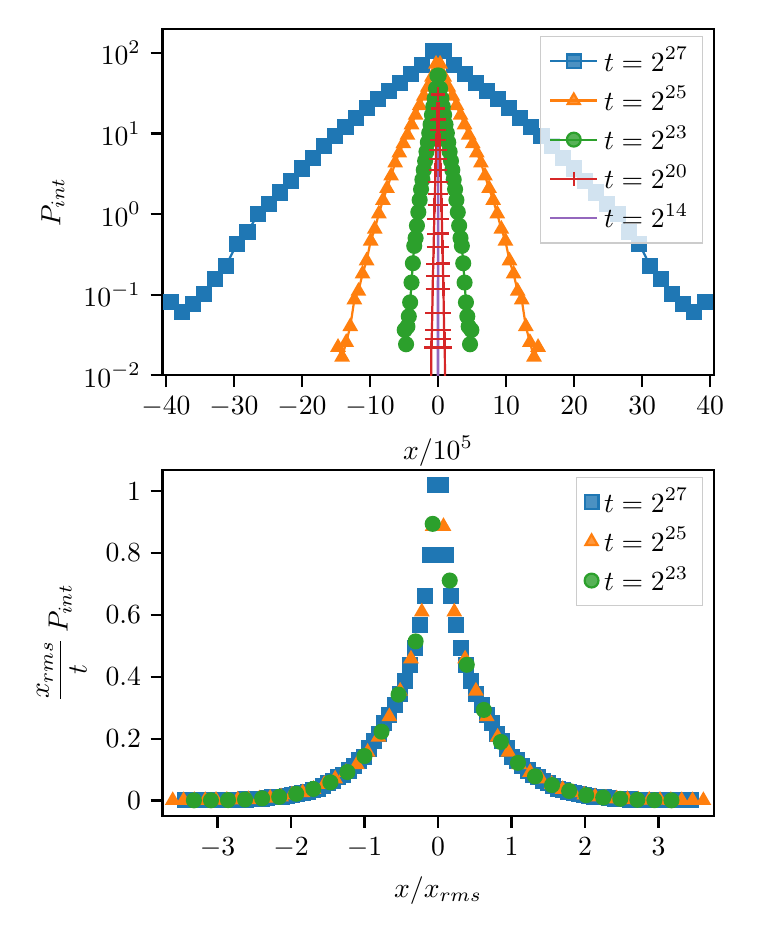
\begin{tikzpicture}

\definecolor{crimson2143940}{RGB}{214,39,40}
\definecolor{darkgrey176}{RGB}{176,176,176}
\definecolor{darkorange25512714}{RGB}{255,127,14}
\definecolor{forestgreen4416044}{RGB}{44,160,44}
\definecolor{lightgrey204}{RGB}{204,204,204}
\definecolor{mediumpurple148103189}{RGB}{148,103,189}
\definecolor{steelblue31119180}{RGB}{31,119,180}

\begin{groupplot}[group style={group size=1 by 2, vertical sep=1.2cm}, width=7cm,height=4.4cm]
\nextgroupplot[
legend cell align={left},
legend style={fill opacity=0.8, draw opacity=1, text opacity=1, draw=lightgrey204},
log basis y={10},
tick align=outside,
tick pos=left,
x grid style={darkgrey176},
xlabel={\(\displaystyle x/10^5\)},
xmin=-40.5, xmax=40.5,
xtick style={color=black},
y grid style={darkgrey176},
ylabel={\(\displaystyle  P_{int} \)},
ymin=0.01, ymax=200.075958407959,
ymode=log,
ytick style={color=black},
ytick={1e-05,0.0001,0.001,0.01,0.1,1,10,100,1000,10000},
yticklabels={
  \(\displaystyle {10^{-5}}\),
  \(\displaystyle {10^{-4}}\),
  \(\displaystyle {10^{-3}}\),
  \(\displaystyle {10^{-2}}\),
  \(\displaystyle {10^{-1}}\),
  \(\displaystyle {10^{0}}\),
  \(\displaystyle {10^{1}}\),
  \(\displaystyle {10^{2}}\),
  \(\displaystyle {10^{3}}\),
  \(\displaystyle {10^{4}}\)
}
]
\addplot [semithick, steelblue31119180, mark=square*, mark size=2.5, mark options={solid}]
table {%
-39.2 0.080824323659419
-37.6 0.0608542550684668
-36 0.0773138489449037
-34.4 0.103299497598756
-32.8 0.155486985682513
-31.2 0.225169950649147
-29.6 0.423077148741531
-28 0.598666251163844
-26.4 1.01708058335806
-24.8 1.3502561561575
-23.2 1.85574374844031
-21.6 2.60965010671125
-20 3.68552583980844
-18.4 5.03078509313844
-16.8 6.96803068676938
-15.2 9.22938250166344
-13.6 12.1783032573487
-12 15.793682929125
-10.4 21.0564022671125
-8.8 27.112895108425
-7.2 34.1099594596375
-5.6 42.7910409872719
-4 54.4652986437594
-2.4 71.7987568989156
-0.8 105.826808965466
0.8 105.826859950441
2.4 71.7987713893531
4 54.4653064644469
5.6 42.7910472490562
7.2 34.10996423035
8.8 27.1128993574219
10.4 21.0564057260469
12 15.7936854098406
13.6 12.1783057352806
15.2 9.22938379105532
16.8 6.96803203743687
18.4 5.03078632793688
20 3.6855263049225
21.6 2.60965086206219
23.2 1.85574400626844
24.8 1.35025642957531
26.4 1.01708086888462
28 0.598666366064469
29.6 0.423077330744781
31.2 0.225170039829856
32.8 0.155486977794647
34.4 0.103299521334869
36 0.0773138761258007
37.6 0.0608542504115826
39.2 0.0807944248535129
};
\addlegendentry{\(\displaystyle t=2^{27}\)}
\addplot [semithick, darkorange25512714, mark=triangle*, mark size=2.5, mark options={solid}]
table {%
-14.7 0.0222840045591143
-14.1 0.0168281545104564
-13.5 0.0256313264836824
-12.9 0.0403175625251967
-12.3 0.0866091064247917
-11.7 0.110561067231
-11.1 0.181332949893267
-10.5 0.263863671570658
-9.9 0.46406832658225
-9.3 0.652293048616667
-8.7 1.01127505399033
-8.1 1.48454785611
-7.5 2.08759996222167
-6.9 2.982874339385
-6.3 4.329841827125
-5.7 5.76267358536083
-5.1 7.5188241264325
-4.5 9.59249497040833
-3.9 12.8966598121
-3.3 16.92634054175
-2.7 22.3516292439583
-2.1 29.1830515198083
-1.5 37.7460184668833
-0.9 50.2760652527333
-0.3 73.0557826509417
0.3 73.0558753159583
0.9 50.2760911324083
1.5 37.7460357959667
2.1 29.1830641029833
2.7 22.3516398714833
3.3 16.92634830845
3.9 12.8966655589667
4.5 9.59250004844917
5.1 7.51882685382583
5.7 5.76267591181833
6.3 4.32984448768
6.9 2.98287648808667
7.5 2.08760083069333
8.1 1.4845487216125
8.7 1.01127572768492
9.3 0.652293661945
9.9 0.464068496357667
10.5 0.263864065666992
11.1 0.181332989642767
11.7 0.1105611811586
12.3 0.0866091413155
12.9 0.04031762029788
13.5 0.0256313369963074
14.1 0.0168281862576014
14.7 0.0222635526133527
};
\addlegendentry{\(\displaystyle t=2^{25}\)}
\addplot [semithick, forestgreen4416044, mark=*, mark size=2.5, mark options={solid}]
table {%
-4.9 0.0364290354472725
-4.7 0.024235335061025
-4.5 0.040259158977075
-4.3 0.053791145130875
-4.1 0.080321032192
-3.9 0.1415827933744
-3.7 0.24578109267175
-3.5 0.403197615127
-3.3 0.50487856551525
-3.1 0.71923106588375
-2.9 1.05802808319975
-2.7 1.49743147097
-2.5 2.0351177840725
-2.3 2.6815934944725
-2.1 3.5277204536
-1.9 4.5806481090075
-1.7 5.9617903031
-1.5 7.789516331915
-1.3 10.16251822212
-1.1 12.981405559975
-0.9 17.065750131275
-0.7 21.65644900135
-0.5 27.24140186805
-0.3 36.2913921503
-0.1 52.521274345525
0.1 52.521467365275
0.3 36.29144841365
0.5 27.241429666375
0.7 21.656479067025
0.9 17.065772052925
1.1 12.981420884875
1.3 10.162532332955
1.5 7.7895269148075
1.7 5.9617979458725
1.9 4.5806544192275
2.1 3.5277244178925
2.3 2.6815970347825
2.5 2.0351204208725
2.7 1.4974347756175
2.9 1.05803000410025
3.1 0.71923202243125
3.3 0.5048794407905
3.5 0.40319865438
3.7 0.24578148621125
3.9 0.141583184476375
4.1 0.080321140060625
4.3 0.05379126883225
4.5 0.040259290463375
4.7 0.0242353954125
4.9 0.0363695941067725
};
\addlegendentry{\(\displaystyle t=2^{23}\)}
\addplot [semithick, crimson2143940, mark=+, mark size=2.5, mark options={solid}]
table {%
-1.184469 0.00031228563923039
-1.136129 0.00192901955133566
-1.087789 0.00364606485537877
-1.039449 0.00448567288593896
-0.991109 0.0220736485715205
-0.942769 0.0279884663211005
-0.894429 0.0363186275863157
-0.846089 0.0594479133501241
-0.797749 0.117372447593504
-0.749409 0.16995828072921
-0.701069 0.242959895920563
-0.652729 0.393460271943525
-0.604389 0.572178636901117
-0.556049 0.864873004212867
-0.507709 1.30960002615846
-0.459369 1.77580569805544
-0.411029 2.49722010468556
-0.362689 3.56204363440215
-0.314349 4.78533828886016
-0.266009 6.29235565449938
-0.217669 8.29296848359537
-0.169329 11.1584978008688
-0.120989 14.9050428476417
-0.072649 20.4628415835747
-0.024309 30.5496883139222
0.024031 30.6829879858295
0.072371 20.5041808772238
0.120711 14.928612796235
0.169051 11.1766462873397
0.217391 8.30821305341332
0.265731 6.30185425634051
0.314071 4.79368651177079
0.362411 3.56720571689077
0.410751 2.50344775154117
0.459091 1.77954280389946
0.507431 1.3115565234278
0.555771 0.867138544915184
0.604111 0.57355002775031
0.652451 0.394540457760654
0.700791 0.243541659121845
0.749131 0.170215842299338
0.797471 0.117710597124017
0.845811 0.0596634482704799
0.894151 0.0363192589956041
0.942491 0.0281253279792615
0.990831 0.0221573534508068
1.039171 0.00450985105555005
1.087511 0.00363779149638622
1.135851 0.00194866960668216
1.184191 0.00031089661512438
};
\addlegendentry{\(\displaystyle t=2^{20}\)}
\addplot [semithick, mediumpurple148103189]
table {%
-0.052956 0.000321985411719907
-0.050796 0.00109559827098356
-0.048636 0.00180578192475718
-0.046476 0.00374894742625
-0.044316 0.00617249055655093
-0.042156 0.00974488099837963
-0.039996 0.0154551167074074
-0.037836 0.0220357126226852
-0.035676 0.0326265787268519
-0.033516 0.0544916889097222
-0.031356 0.0974713543333333
-0.029196 0.137497860886574
-0.027036 0.199152393009259
-0.024876 0.289246719398148
-0.022716 0.447956153148148
-0.020556 0.59892095037037
-0.018396 0.828516219976852
-0.016236 1.19865974594907
-0.014076 1.65238581921296
-0.011916 2.17833360555556
-0.009756 2.87499786134259
-0.007596 3.96499589027778
-0.005436 5.26300859282407
-0.003276 7.12862474097222
-0.001116 10.5841887574074
0.001044 10.8180993599537
0.003204 7.21165687013889
0.005364 5.31110190949074
0.007524 4.00489944305556
0.009684 2.90688390740741
0.011844 2.19865974166667
0.014004 1.66516002939815
0.016164 1.21548545023148
0.018324 0.837138882083333
0.020484 0.606186718148148
0.022644 0.452229408356482
0.024804 0.293560020046296
0.026964 0.202202421736111
0.029124 0.138803387460648
0.031284 0.0989739992152778
0.033444 0.0556306353310185
0.035604 0.0331923876412037
0.037764 0.0221578228773148
0.039924 0.01547282555
0.042084 0.0101039635333333
0.044244 0.00620626870840278
0.046404 0.00396959774613426
0.048564 0.00181247479696319
0.050724 0.00109336141893958
0.052884 0.000346785002453704
};
\addlegendentry{\(\displaystyle t=2^{14}\)}

\nextgroupplot[
legend cell align={left},
legend style={fill opacity=0.8, draw opacity=1, text opacity=1, draw=lightgrey204},
tick align=outside,
tick pos=left,
x grid style={darkgrey176},
xlabel={\(\displaystyle x / x_{rms}\)},
xmin=-3.75, xmax=3.75,
xtick style={color=black},
y grid style={darkgrey176},
ylabel={\(\displaystyle  \frac{x_{rms}}{t} \, P_{int}\)},
ymin=-0.0507159808870153, ymax=1.06952783136885,
ytick style={color=black}
]
\addplot [semithick, steelblue31119180, mark=square*, mark size=2.5, mark options={solid}, only marks]
table {%
-3.44571968472946 0.000966472792408415
-3.37610918604805 0.000417658967078003
-3.30649868736665 0.000504457043121159
-3.23688818868525 0.000537683531974594
-3.16727769000384 0.000494955997052486
-3.09766719132244 0.000829058222029763
-3.02805669264104 0.000771619043989384
-2.95844619395963 0.000997404300615701
-2.88883569527823 0.00118904277687465
-2.81922519659683 0.00147370112651828
-2.74961469791542 0.00188229545779283
-2.68000419923402 0.00197378233988574
-2.61039370055262 0.00316864366013826
-2.54078320187122 0.00407663216491801
-2.47117270318981 0.00472694935274213
-2.40156220450841 0.00552532290950749
-2.33195170582701 0.00749005477656969
-2.2623412071456 0.00992764169949365
-2.1927307084642 0.0108373626396521
-2.1231202097828 0.0122860282476633
-2.05350971110139 0.014599443865993
-1.98389921241999 0.0171805172074613
-1.91428871373859 0.0199450379633142
-1.84467821505718 0.0247457114336987
-1.77506771637578 0.0288241116341348
-1.70545721769438 0.0342912122476038
-1.63584671901297 0.0386906485742961
-1.56623622033157 0.0474624932930687
-1.49662572165017 0.0554759730080668
-1.42701522296876 0.0638528643760178
-1.35740472428736 0.0745044221700129
-1.28779422560596 0.0835504907894948
-1.21818372692456 0.0969540162323974
-1.14857322824315 0.111601719862388
-1.07896272956175 0.129305539623004
-1.00935223088035 0.141164254019529
-0.939741732198943 0.16810027275069
-0.87013123351754 0.192494580368576
-0.800520734836136 0.214589380139683
-0.730910236154733 0.249724053144724
-0.66129973747333 0.276855856798913
-0.591689238791927 0.307283620839344
-0.522078740110524 0.34496749511369
-0.452468241429121 0.387837138075043
-0.382857742747717 0.438947151077044
-0.313247244066314 0.493781342394914
-0.243636745384911 0.567905607230526
-0.174026246703508 0.661661622236197
-0.104415748022105 0.79369703335266
-0.0348052493407016 1.01860699422497
0.0348052493407016 1.0186076580845
0.104415748022105 0.793697242620428
0.174026246703508 0.661661759318833
0.243636745384911 0.56790571829936
0.313247244066314 0.493781406584721
0.382857742747717 0.438947220817982
0.452468241429121 0.387837198031719
0.522078740110524 0.34496754239125
0.591689238791927 0.3072836672942
0.66129973747333 0.276855892043406
0.730910236154733 0.249724088226314
0.800520734836136 0.214589417822964
0.87013123351754 0.192494605381412
0.939741732198943 0.168100306972756
1.00935223088035 0.141164277207891
1.07896272956175 0.129305558917365
1.14857322824315 0.111601738051799
1.21818372692456 0.0969540404780356
1.28779422560596 0.0835505033650825
1.35740472428736 0.0745044316755038
1.42701522296876 0.063852878387804
1.49662572165017 0.0554759821267158
1.56623622033157 0.0474625047426967
1.63584671901297 0.0386906582708239
1.70545721769438 0.0342912160352673
1.77506771637578 0.0288241158116372
1.84467821505718 0.0247457195775124
1.91428871373859 0.0199450427550275
1.98389921241999 0.0171805187279265
2.05350971110139 0.014599446760883
2.1231202097828 0.0122860311103312
2.1927307084642 0.0108373644593158
2.2623412071456 0.00992764345415007
2.33195170582701 0.0074900579116094
2.40156220450841 0.00552532433557918
2.47117270318981 0.00472694989436527
2.54078320187122 0.00407663371760157
2.61039370055262 0.00316864522429462
2.68000419923402 0.001973782766304
2.74961469791542 0.00188229655861101
2.81922519659683 0.0014737010521377
2.88883569527823 0.00118904271617405
2.95844619395963 0.000997404417635859
3.02805669264104 0.000771619333454621
3.09766719132244 0.000829058924755227
3.16727769000384 0.000494955759804998
3.23688818868525 0.000537683739272804
3.30649868736665 0.000504456756072928
3.37610918604805 0.00041765904264311
3.44571968472946 0.000965960694163107
};
\addlegendentry{\(\displaystyle t=2^{27}\)}
\addplot [semithick, darkorange25512714, mark=triangle*, mark size=2.5, mark options={solid}, only marks]
table {%
-3.61047519831227 0.000270393542588787
-3.46310886368728 0.000204192397342367
-3.31574252906229 0.000311009861391275
-3.1683761944373 0.000489212274697458
-3.02100985981231 0.00105091268692414
-2.87364352518732 0.00134154516804565
-2.72627719056233 0.00220028938603233
-2.57891085593734 0.0032017150565199
-2.43154452131235 0.00563099323081506
-2.28417818668736 0.00791490720411656
-2.13681185206236 0.0122707856953957
-1.98944551743737 0.0180134657974655
-1.84207918281238 0.0253308846619518
-1.69471284818739 0.0361941211052936
-1.5473465135624 0.0525381902242784
-1.39998017893741 0.069924134210035
-1.25261384431242 0.0912332200549921
-1.10524750968743 0.116395089151647
-0.957881175062439 0.156487741011966
-0.810514840437449 0.205383784140183
-0.663148505812458 0.27121409878877
-0.515782171187467 0.354106402332637
-0.368415836562477 0.458009224724732
-0.221049501937486 0.610048492632865
-0.0736831673124953 0.886457002159654
0.0736831673124953 0.886458126554601
0.221049501937486 0.610048806656181
0.368415836562477 0.458009434995388
0.515782171187467 0.354106555016561
0.663148505812458 0.271214227742886
0.810514840437449 0.205383878381122
0.957881175062439 0.1564878107443
1.10524750968743 0.116395150768465
1.25261384431242 0.0912332531491132
1.39998017893741 0.0699241624392109
1.5473465135624 0.0525382225073848
1.69471284818739 0.0361941471775847
1.84207918281238 0.0253308951999649
1.98944551743737 0.0180134762994508
2.13681185206236 0.0122707938699886
2.28417818668736 0.0079149146462269
2.43154452131235 0.00563099529086564
2.57891085593734 0.00320171983847475
2.72627719056233 0.00220028986835175
2.87364352518732 0.00134154655044024
3.02100985981231 0.00105091311028711
3.1683761944373 0.000489212975709723
3.31574252906229 0.000311009988951198
3.46310886368728 0.000204192782561414
3.61047519831227 0.000270145379200889
};
\addlegendentry{\(\displaystyle t=2^{25}\)}
\addplot [semithick, forestgreen4416044, mark=*, mark size=2.5, mark options={solid}, only marks]
table {%
-3.3222558508543 0.000537445611094879
-3.0901707073276 0.000683726022316047
-2.85808556380091 0.0012595508884797
-2.62600042027422 0.00325743103700495
-2.39391527674753 0.00692196888565562
-2.16183013322084 0.0116400815731717
-1.92974498969415 0.0217236449310345
-1.69765984616746 0.0373172634040754
-1.46557470264077 0.0586627771073573
-1.23348955911408 0.091935978787301
-1.00140441558739 0.14363033312385
-0.769319272060697 0.222483289335882
-0.537234128534006 0.342315781222818
-0.305148985007316 0.51448487032096
-0.0730638414806249 0.894452486127128
0.159021302046066 0.711193303722155
0.391106445572757 0.438767628173372
0.623191589099447 0.292844246722494
0.855276732626138 0.189261782711863
1.08736187615283 0.121677111641111
1.31944701967952 0.078074528713982
1.55153216320621 0.0498938248731224
1.7836173067329 0.030793480903353
2.01570245025959 0.0172705947178269
2.24778759378628 0.00957547508127624
2.47987273731297 0.00544179286020076
2.71195788083966 0.00223040154254092
2.94404302436635 0.00102209288294553
3.17612816789305 0.000527860175812559
};
\addlegendentry{\(\displaystyle t=2^{23}\)}
\end{groupplot}

\end{tikzpicture}

    \caption{Here is sample caption to match to the figure text size to the caption text size.}
\end{figure}
% 
% \vfill

\newpage

\begin{figure}
    \centering
    % This file was created with tikzplotlib v0.10.1.post13.
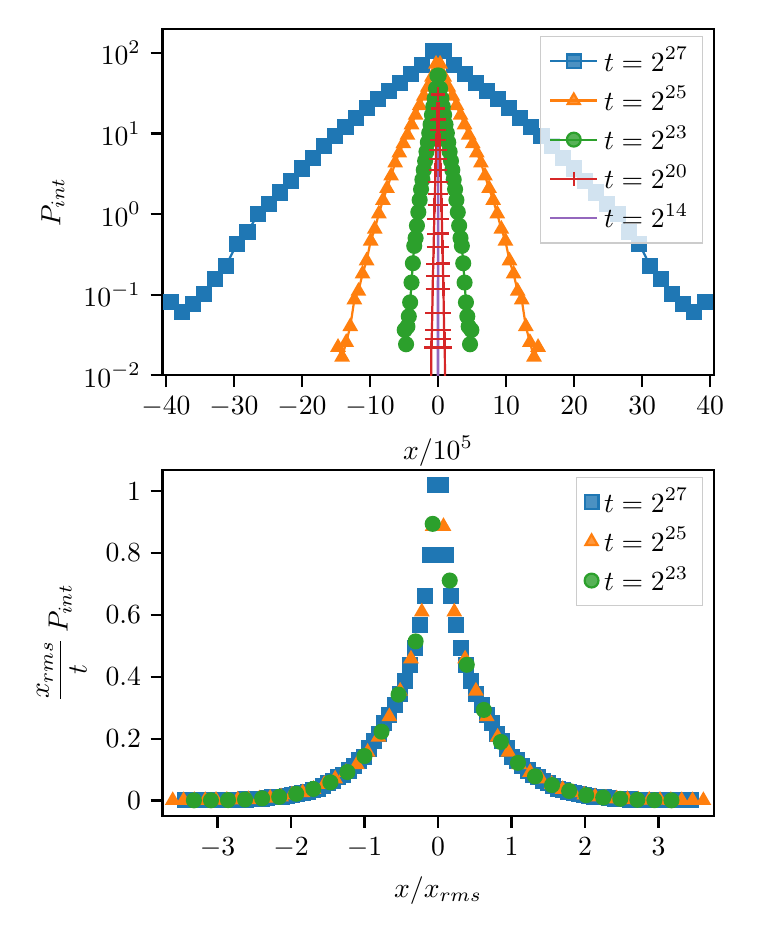
\begin{tikzpicture}

\definecolor{crimson2143940}{RGB}{214,39,40}
\definecolor{darkgrey176}{RGB}{176,176,176}
\definecolor{darkorange25512714}{RGB}{255,127,14}
\definecolor{forestgreen4416044}{RGB}{44,160,44}
\definecolor{lightgrey204}{RGB}{204,204,204}
\definecolor{mediumpurple148103189}{RGB}{148,103,189}
\definecolor{steelblue31119180}{RGB}{31,119,180}

\begin{groupplot}[group style={group size=1 by 2, vertical sep=1.2cm}, width=7cm,height=4.4cm]
\nextgroupplot[
legend cell align={left},
legend style={fill opacity=0.8, draw opacity=1, text opacity=1, draw=lightgrey204},
log basis y={10},
tick align=outside,
tick pos=left,
x grid style={darkgrey176},
xlabel={\(\displaystyle x/10^5\)},
xmin=-40.5, xmax=40.5,
xtick style={color=black},
y grid style={darkgrey176},
ylabel={\(\displaystyle  P_{int} \)},
ymin=0.01, ymax=200.075958407959,
ymode=log,
ytick style={color=black},
ytick={1e-05,0.0001,0.001,0.01,0.1,1,10,100,1000,10000},
yticklabels={
  \(\displaystyle {10^{-5}}\),
  \(\displaystyle {10^{-4}}\),
  \(\displaystyle {10^{-3}}\),
  \(\displaystyle {10^{-2}}\),
  \(\displaystyle {10^{-1}}\),
  \(\displaystyle {10^{0}}\),
  \(\displaystyle {10^{1}}\),
  \(\displaystyle {10^{2}}\),
  \(\displaystyle {10^{3}}\),
  \(\displaystyle {10^{4}}\)
}
]
\addplot [semithick, steelblue31119180, mark=square*, mark size=2.5, mark options={solid}]
table {%
-39.2 0.080824323659419
-37.6 0.0608542550684668
-36 0.0773138489449037
-34.4 0.103299497598756
-32.8 0.155486985682513
-31.2 0.225169950649147
-29.6 0.423077148741531
-28 0.598666251163844
-26.4 1.01708058335806
-24.8 1.3502561561575
-23.2 1.85574374844031
-21.6 2.60965010671125
-20 3.68552583980844
-18.4 5.03078509313844
-16.8 6.96803068676938
-15.2 9.22938250166344
-13.6 12.1783032573487
-12 15.793682929125
-10.4 21.0564022671125
-8.8 27.112895108425
-7.2 34.1099594596375
-5.6 42.7910409872719
-4 54.4652986437594
-2.4 71.7987568989156
-0.8 105.826808965466
0.8 105.826859950441
2.4 71.7987713893531
4 54.4653064644469
5.6 42.7910472490562
7.2 34.10996423035
8.8 27.1128993574219
10.4 21.0564057260469
12 15.7936854098406
13.6 12.1783057352806
15.2 9.22938379105532
16.8 6.96803203743687
18.4 5.03078632793688
20 3.6855263049225
21.6 2.60965086206219
23.2 1.85574400626844
24.8 1.35025642957531
26.4 1.01708086888462
28 0.598666366064469
29.6 0.423077330744781
31.2 0.225170039829856
32.8 0.155486977794647
34.4 0.103299521334869
36 0.0773138761258007
37.6 0.0608542504115826
39.2 0.0807944248535129
};
\addlegendentry{\(\displaystyle t=2^{27}\)}
\addplot [semithick, darkorange25512714, mark=triangle*, mark size=2.5, mark options={solid}]
table {%
-14.7 0.0222840045591143
-14.1 0.0168281545104564
-13.5 0.0256313264836824
-12.9 0.0403175625251967
-12.3 0.0866091064247917
-11.7 0.110561067231
-11.1 0.181332949893267
-10.5 0.263863671570658
-9.9 0.46406832658225
-9.3 0.652293048616667
-8.7 1.01127505399033
-8.1 1.48454785611
-7.5 2.08759996222167
-6.9 2.982874339385
-6.3 4.329841827125
-5.7 5.76267358536083
-5.1 7.5188241264325
-4.5 9.59249497040833
-3.9 12.8966598121
-3.3 16.92634054175
-2.7 22.3516292439583
-2.1 29.1830515198083
-1.5 37.7460184668833
-0.9 50.2760652527333
-0.3 73.0557826509417
0.3 73.0558753159583
0.9 50.2760911324083
1.5 37.7460357959667
2.1 29.1830641029833
2.7 22.3516398714833
3.3 16.92634830845
3.9 12.8966655589667
4.5 9.59250004844917
5.1 7.51882685382583
5.7 5.76267591181833
6.3 4.32984448768
6.9 2.98287648808667
7.5 2.08760083069333
8.1 1.4845487216125
8.7 1.01127572768492
9.3 0.652293661945
9.9 0.464068496357667
10.5 0.263864065666992
11.1 0.181332989642767
11.7 0.1105611811586
12.3 0.0866091413155
12.9 0.04031762029788
13.5 0.0256313369963074
14.1 0.0168281862576014
14.7 0.0222635526133527
};
\addlegendentry{\(\displaystyle t=2^{25}\)}
\addplot [semithick, forestgreen4416044, mark=*, mark size=2.5, mark options={solid}]
table {%
-4.9 0.0364290354472725
-4.7 0.024235335061025
-4.5 0.040259158977075
-4.3 0.053791145130875
-4.1 0.080321032192
-3.9 0.1415827933744
-3.7 0.24578109267175
-3.5 0.403197615127
-3.3 0.50487856551525
-3.1 0.71923106588375
-2.9 1.05802808319975
-2.7 1.49743147097
-2.5 2.0351177840725
-2.3 2.6815934944725
-2.1 3.5277204536
-1.9 4.5806481090075
-1.7 5.9617903031
-1.5 7.789516331915
-1.3 10.16251822212
-1.1 12.981405559975
-0.9 17.065750131275
-0.7 21.65644900135
-0.5 27.24140186805
-0.3 36.2913921503
-0.1 52.521274345525
0.1 52.521467365275
0.3 36.29144841365
0.5 27.241429666375
0.7 21.656479067025
0.9 17.065772052925
1.1 12.981420884875
1.3 10.162532332955
1.5 7.7895269148075
1.7 5.9617979458725
1.9 4.5806544192275
2.1 3.5277244178925
2.3 2.6815970347825
2.5 2.0351204208725
2.7 1.4974347756175
2.9 1.05803000410025
3.1 0.71923202243125
3.3 0.5048794407905
3.5 0.40319865438
3.7 0.24578148621125
3.9 0.141583184476375
4.1 0.080321140060625
4.3 0.05379126883225
4.5 0.040259290463375
4.7 0.0242353954125
4.9 0.0363695941067725
};
\addlegendentry{\(\displaystyle t=2^{23}\)}
\addplot [semithick, crimson2143940, mark=+, mark size=2.5, mark options={solid}]
table {%
-1.184469 0.00031228563923039
-1.136129 0.00192901955133566
-1.087789 0.00364606485537877
-1.039449 0.00448567288593896
-0.991109 0.0220736485715205
-0.942769 0.0279884663211005
-0.894429 0.0363186275863157
-0.846089 0.0594479133501241
-0.797749 0.117372447593504
-0.749409 0.16995828072921
-0.701069 0.242959895920563
-0.652729 0.393460271943525
-0.604389 0.572178636901117
-0.556049 0.864873004212867
-0.507709 1.30960002615846
-0.459369 1.77580569805544
-0.411029 2.49722010468556
-0.362689 3.56204363440215
-0.314349 4.78533828886016
-0.266009 6.29235565449938
-0.217669 8.29296848359537
-0.169329 11.1584978008688
-0.120989 14.9050428476417
-0.072649 20.4628415835747
-0.024309 30.5496883139222
0.024031 30.6829879858295
0.072371 20.5041808772238
0.120711 14.928612796235
0.169051 11.1766462873397
0.217391 8.30821305341332
0.265731 6.30185425634051
0.314071 4.79368651177079
0.362411 3.56720571689077
0.410751 2.50344775154117
0.459091 1.77954280389946
0.507431 1.3115565234278
0.555771 0.867138544915184
0.604111 0.57355002775031
0.652451 0.394540457760654
0.700791 0.243541659121845
0.749131 0.170215842299338
0.797471 0.117710597124017
0.845811 0.0596634482704799
0.894151 0.0363192589956041
0.942491 0.0281253279792615
0.990831 0.0221573534508068
1.039171 0.00450985105555005
1.087511 0.00363779149638622
1.135851 0.00194866960668216
1.184191 0.00031089661512438
};
\addlegendentry{\(\displaystyle t=2^{20}\)}
\addplot [semithick, mediumpurple148103189]
table {%
-0.052956 0.000321985411719907
-0.050796 0.00109559827098356
-0.048636 0.00180578192475718
-0.046476 0.00374894742625
-0.044316 0.00617249055655093
-0.042156 0.00974488099837963
-0.039996 0.0154551167074074
-0.037836 0.0220357126226852
-0.035676 0.0326265787268519
-0.033516 0.0544916889097222
-0.031356 0.0974713543333333
-0.029196 0.137497860886574
-0.027036 0.199152393009259
-0.024876 0.289246719398148
-0.022716 0.447956153148148
-0.020556 0.59892095037037
-0.018396 0.828516219976852
-0.016236 1.19865974594907
-0.014076 1.65238581921296
-0.011916 2.17833360555556
-0.009756 2.87499786134259
-0.007596 3.96499589027778
-0.005436 5.26300859282407
-0.003276 7.12862474097222
-0.001116 10.5841887574074
0.001044 10.8180993599537
0.003204 7.21165687013889
0.005364 5.31110190949074
0.007524 4.00489944305556
0.009684 2.90688390740741
0.011844 2.19865974166667
0.014004 1.66516002939815
0.016164 1.21548545023148
0.018324 0.837138882083333
0.020484 0.606186718148148
0.022644 0.452229408356482
0.024804 0.293560020046296
0.026964 0.202202421736111
0.029124 0.138803387460648
0.031284 0.0989739992152778
0.033444 0.0556306353310185
0.035604 0.0331923876412037
0.037764 0.0221578228773148
0.039924 0.01547282555
0.042084 0.0101039635333333
0.044244 0.00620626870840278
0.046404 0.00396959774613426
0.048564 0.00181247479696319
0.050724 0.00109336141893958
0.052884 0.000346785002453704
};
\addlegendentry{\(\displaystyle t=2^{14}\)}

\nextgroupplot[
legend cell align={left},
legend style={fill opacity=0.8, draw opacity=1, text opacity=1, draw=lightgrey204},
tick align=outside,
tick pos=left,
x grid style={darkgrey176},
xlabel={\(\displaystyle x / x_{rms}\)},
xmin=-3.75, xmax=3.75,
xtick style={color=black},
y grid style={darkgrey176},
ylabel={\(\displaystyle  \frac{x_{rms}}{t} \, P_{int}\)},
ymin=-0.0507159808870153, ymax=1.06952783136885,
ytick style={color=black}
]
\addplot [semithick, steelblue31119180, mark=square*, mark size=2.5, mark options={solid}, only marks]
table {%
-3.44571968472946 0.000966472792408415
-3.37610918604805 0.000417658967078003
-3.30649868736665 0.000504457043121159
-3.23688818868525 0.000537683531974594
-3.16727769000384 0.000494955997052486
-3.09766719132244 0.000829058222029763
-3.02805669264104 0.000771619043989384
-2.95844619395963 0.000997404300615701
-2.88883569527823 0.00118904277687465
-2.81922519659683 0.00147370112651828
-2.74961469791542 0.00188229545779283
-2.68000419923402 0.00197378233988574
-2.61039370055262 0.00316864366013826
-2.54078320187122 0.00407663216491801
-2.47117270318981 0.00472694935274213
-2.40156220450841 0.00552532290950749
-2.33195170582701 0.00749005477656969
-2.2623412071456 0.00992764169949365
-2.1927307084642 0.0108373626396521
-2.1231202097828 0.0122860282476633
-2.05350971110139 0.014599443865993
-1.98389921241999 0.0171805172074613
-1.91428871373859 0.0199450379633142
-1.84467821505718 0.0247457114336987
-1.77506771637578 0.0288241116341348
-1.70545721769438 0.0342912122476038
-1.63584671901297 0.0386906485742961
-1.56623622033157 0.0474624932930687
-1.49662572165017 0.0554759730080668
-1.42701522296876 0.0638528643760178
-1.35740472428736 0.0745044221700129
-1.28779422560596 0.0835504907894948
-1.21818372692456 0.0969540162323974
-1.14857322824315 0.111601719862388
-1.07896272956175 0.129305539623004
-1.00935223088035 0.141164254019529
-0.939741732198943 0.16810027275069
-0.87013123351754 0.192494580368576
-0.800520734836136 0.214589380139683
-0.730910236154733 0.249724053144724
-0.66129973747333 0.276855856798913
-0.591689238791927 0.307283620839344
-0.522078740110524 0.34496749511369
-0.452468241429121 0.387837138075043
-0.382857742747717 0.438947151077044
-0.313247244066314 0.493781342394914
-0.243636745384911 0.567905607230526
-0.174026246703508 0.661661622236197
-0.104415748022105 0.79369703335266
-0.0348052493407016 1.01860699422497
0.0348052493407016 1.0186076580845
0.104415748022105 0.793697242620428
0.174026246703508 0.661661759318833
0.243636745384911 0.56790571829936
0.313247244066314 0.493781406584721
0.382857742747717 0.438947220817982
0.452468241429121 0.387837198031719
0.522078740110524 0.34496754239125
0.591689238791927 0.3072836672942
0.66129973747333 0.276855892043406
0.730910236154733 0.249724088226314
0.800520734836136 0.214589417822964
0.87013123351754 0.192494605381412
0.939741732198943 0.168100306972756
1.00935223088035 0.141164277207891
1.07896272956175 0.129305558917365
1.14857322824315 0.111601738051799
1.21818372692456 0.0969540404780356
1.28779422560596 0.0835505033650825
1.35740472428736 0.0745044316755038
1.42701522296876 0.063852878387804
1.49662572165017 0.0554759821267158
1.56623622033157 0.0474625047426967
1.63584671901297 0.0386906582708239
1.70545721769438 0.0342912160352673
1.77506771637578 0.0288241158116372
1.84467821505718 0.0247457195775124
1.91428871373859 0.0199450427550275
1.98389921241999 0.0171805187279265
2.05350971110139 0.014599446760883
2.1231202097828 0.0122860311103312
2.1927307084642 0.0108373644593158
2.2623412071456 0.00992764345415007
2.33195170582701 0.0074900579116094
2.40156220450841 0.00552532433557918
2.47117270318981 0.00472694989436527
2.54078320187122 0.00407663371760157
2.61039370055262 0.00316864522429462
2.68000419923402 0.001973782766304
2.74961469791542 0.00188229655861101
2.81922519659683 0.0014737010521377
2.88883569527823 0.00118904271617405
2.95844619395963 0.000997404417635859
3.02805669264104 0.000771619333454621
3.09766719132244 0.000829058924755227
3.16727769000384 0.000494955759804998
3.23688818868525 0.000537683739272804
3.30649868736665 0.000504456756072928
3.37610918604805 0.00041765904264311
3.44571968472946 0.000965960694163107
};
\addlegendentry{\(\displaystyle t=2^{27}\)}
\addplot [semithick, darkorange25512714, mark=triangle*, mark size=2.5, mark options={solid}, only marks]
table {%
-3.61047519831227 0.000270393542588787
-3.46310886368728 0.000204192397342367
-3.31574252906229 0.000311009861391275
-3.1683761944373 0.000489212274697458
-3.02100985981231 0.00105091268692414
-2.87364352518732 0.00134154516804565
-2.72627719056233 0.00220028938603233
-2.57891085593734 0.0032017150565199
-2.43154452131235 0.00563099323081506
-2.28417818668736 0.00791490720411656
-2.13681185206236 0.0122707856953957
-1.98944551743737 0.0180134657974655
-1.84207918281238 0.0253308846619518
-1.69471284818739 0.0361941211052936
-1.5473465135624 0.0525381902242784
-1.39998017893741 0.069924134210035
-1.25261384431242 0.0912332200549921
-1.10524750968743 0.116395089151647
-0.957881175062439 0.156487741011966
-0.810514840437449 0.205383784140183
-0.663148505812458 0.27121409878877
-0.515782171187467 0.354106402332637
-0.368415836562477 0.458009224724732
-0.221049501937486 0.610048492632865
-0.0736831673124953 0.886457002159654
0.0736831673124953 0.886458126554601
0.221049501937486 0.610048806656181
0.368415836562477 0.458009434995388
0.515782171187467 0.354106555016561
0.663148505812458 0.271214227742886
0.810514840437449 0.205383878381122
0.957881175062439 0.1564878107443
1.10524750968743 0.116395150768465
1.25261384431242 0.0912332531491132
1.39998017893741 0.0699241624392109
1.5473465135624 0.0525382225073848
1.69471284818739 0.0361941471775847
1.84207918281238 0.0253308951999649
1.98944551743737 0.0180134762994508
2.13681185206236 0.0122707938699886
2.28417818668736 0.0079149146462269
2.43154452131235 0.00563099529086564
2.57891085593734 0.00320171983847475
2.72627719056233 0.00220028986835175
2.87364352518732 0.00134154655044024
3.02100985981231 0.00105091311028711
3.1683761944373 0.000489212975709723
3.31574252906229 0.000311009988951198
3.46310886368728 0.000204192782561414
3.61047519831227 0.000270145379200889
};
\addlegendentry{\(\displaystyle t=2^{25}\)}
\addplot [semithick, forestgreen4416044, mark=*, mark size=2.5, mark options={solid}, only marks]
table {%
-3.3222558508543 0.000537445611094879
-3.0901707073276 0.000683726022316047
-2.85808556380091 0.0012595508884797
-2.62600042027422 0.00325743103700495
-2.39391527674753 0.00692196888565562
-2.16183013322084 0.0116400815731717
-1.92974498969415 0.0217236449310345
-1.69765984616746 0.0373172634040754
-1.46557470264077 0.0586627771073573
-1.23348955911408 0.091935978787301
-1.00140441558739 0.14363033312385
-0.769319272060697 0.222483289335882
-0.537234128534006 0.342315781222818
-0.305148985007316 0.51448487032096
-0.0730638414806249 0.894452486127128
0.159021302046066 0.711193303722155
0.391106445572757 0.438767628173372
0.623191589099447 0.292844246722494
0.855276732626138 0.189261782711863
1.08736187615283 0.121677111641111
1.31944701967952 0.078074528713982
1.55153216320621 0.0498938248731224
1.7836173067329 0.030793480903353
2.01570245025959 0.0172705947178269
2.24778759378628 0.00957547508127624
2.47987273731297 0.00544179286020076
2.71195788083966 0.00223040154254092
2.94404302436635 0.00102209288294553
3.17612816789305 0.000527860175812559
};
\addlegendentry{\(\displaystyle t=2^{23}\)}
\end{groupplot}

\end{tikzpicture}

    \caption{Here is sample caption to match to the figure text size to the caption text size.}
\end{figure}

\end{document}